\documentclass[preprint]{revtex4-2}
\usepackage[utf8]{inputenc}
\usepackage{kotex}
\usepackage{amsmath}
\usepackage{amssymb}
\usepackage{amsfonts}
\usepackage{graphicx}
\graphicspath{ {./images/} }
\usepackage{dcolumn}
\usepackage{bm}
\usepackage{hyperref}
\usepackage{mathptmx}
\usepackage{tikz}
\usetikzlibrary{positioning}
\usepackage{textcomp}
\usepackage{natbib}
\usepackage[rightcaption]{sidecap}
\usepackage{wrapfig}



\begin{document}

\title{common sense}
\author{박석훈}
\date{May 2022}


\section{들어가며}
안녕하세요? 6월 시사상식이 나올 때쯤이면 여러분들께서 이 글을 볼 수 있을 것이라고 생각합니다... 이번 시사상식 컨셉은 재블린 미사일과 ICBM입니다. 살상 범위에 따라서 구분해봤어요. 

\section{단거리미사일}

이것도 2가지 분류로 나눠서

\subsection{유류세 인하}

정부는 5월부터 유류세 인하 폭을 30\%로 확대한다. 생계형 경유 사용자에게는 유가 연동 보조금을 지급해 유류비 부담을 낮춘다. 20\%인 유류세 인하 폭은 30\%로 확대되었으며, 경유를 사용하는 영업용 화물차, 버스, 연안 화물선 등에 대해서는 유가연동 보조금을 지급한다.

유류세 인하와 관련하여 소개할 것은 소비자물가지수\footnote{소비자물가지수란 가구에서 일상소비생활을 영위하기 위해 구입하는 상품과 서비스의 가격변동을 측정하기 위하여 작성한 지수를 의미한다.}이다. 통계청에서는 매월 지역별로 소비자물가지수를 발표하고 있다. 이름이 직관적이고 숫자도 깔끔해보여 사람들의 심리를 뒤흔들기 좋다는 것이 특징이다. 2022년 5월달에는 의안정보시스템에 2022년도 농산물가격안정기금운용계획변경안을 제외하고는 아직까지 관련된 의안이 올라오지도 않았고, 계류상태이니 이번 기회로 새로운 의안들이 있는지 확인해보는 계기로 삼아보겠습니다.

유류세에는 교육세, 지방주행세, 교통에너지환경세 크게 세 가지가 있습니다. 이중 가장 큰 비중을 차지하는 세금은 교통에너지환경세로 전체 유류세의 절반 이상을 차지하고 있다. 또한, 전국 기름값을 확인하는 방법으로는 한국석유공사에서 운영하는 오피넷 사이트가 있다. 지역별 평균, 최소, 최대 가격을 일 단위별로 올려주는 사이트이고, 언론에서 가장 많이 인용하는 사이트 중 하나이다. 유류세 인하 폭을 30\%로 확대하면, 약 L당 80원 정도의 세금이 경감된다. 실제 세금 인하 효과를 보기까지는 약 2~3주 정도 걸릴 것으로 예상된다. 그 이유는 유류세 인하가 정유공장 출고를 기준으로 적용되기 때문에, 실제 주유소에 적용되기까지 시간이 소요되기 때문이다. \\

[Fig 1] 소비자물가상승률\\
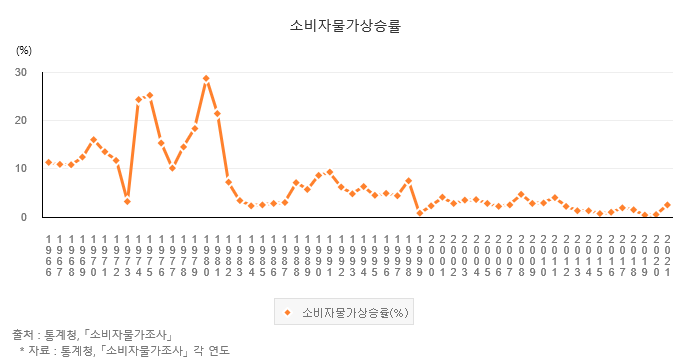
\includegraphics[width=\textwidth]{images/price.png} \\

\subsection{검수완박}
그냥 안넣기는 그렇고. 검찰 수사권 완전 박탈의 줄임말입니다. 검찰의 수사기능을 없애고 기소 및 공소 유지 기능만 담당하는 것을 목표로 합니다. 어째어째 싸우면서 뒤로 이상한거 통과시켰을텐데 그게 뭔질 모르겠네요. 어쨌든 통과되었고 저도 잘 모릅니다.

\subsection{마이데이터}
빅데이터 활용을 위한 개인정보 비식별화 사례집, 금융 마이데이터 서비스 가이드라인, 금융 마이데이터 기술 가이드라인, 개인정보의 안전성 확보조치 기준 및 해설서, 개인정보 보호 법령 및 지침 고시 해설서 등등...

얘네 좀 잘 넣어서 가능?

\subsection{지방소멸}
통계청에 따르면 한국의 수도권(서울, 경기, 인천) 인구가 비수도권 인구를 처음으로 초과했다고 한다. 국토면적의 12\% 정도인 수도권에 과반의 인구가 모여있다는 것을 의미하며, 수도권의 인구 과밀은 곧 지방의 인구 급감과 맞닿아 있는 문제이다. 서울대학교 경제학부 이철희 교수의 연구에 따르면, 지역 간 인구불균등 확대는 거의 전적으로 하위 시군구 인구의 상대적인 감소에 의해 발생한 것으로 파악된다. 또한, 연령별로 수행한 분석 결과는 특히 20-39세 인구 이동률의 시군구 간 차이가 지자체 간 인구불균형 확대를 주된 요인이었음을 보여준다.

국토연구원 국토이슈리포트 57호에서는 인구의 자연적 감소(출산율 감소)보다 사회적 감소(인구 이동)이 더 큰 요인으로 지적하고 있다. 따라서 기존의 저출산 대책으로 지방소멸 위기에 대응하는 것으로는 부족하며 지역 단위의 전략적 사업을 연계 및 통합할 것을 제안한다. 예를 들어, 부산과 울산 경남을 하나로 묶는 `동남권 메가시티'와 같은 것들이 대표적이다. 지역 통합의 문제... 메가시티 등등... 여기서 왜 묶는지 정도만 설명하고 넘어가기(*별로 안중요)

\subsection{장애인 이동권}





\section{ICBM미사일들}

일정한 흐름을 기준으로 전개.

\subsection{시멘트수급}

\subsection{SCI 논문}

\subsection{블록화}

\subsection{ICBM 미사일 발사}

\subsection{EU 패스트패션}

양식변경

\end{document}
